\chapter{Diskusia: problémy a kam ďalej}
\label{chap:future-works}

V poslednej kapitole by sme radi čitateľa hlbšie zasvätili do problémov, na ktoré sme narazili, častiach, ktoré sme z práce vypustili a námetov na ďalšie
skúmanie či na témy záverečných prác

\section{Zapracovanie návodu do používateľského rozhrania}
Ako sme už v úvode zdôraznili, nepodarilo sa nám nájsť zmysluplný spôsob, ako vložiť vedomosti a popis do systému. V konečnom dôsledku si myslíme,
že to nie je problém, pretože m-KIB môže čerpať vedomosti z kapitol \ref{chap:it-grundschutz} a \ref{chap:risk-analysis}. Používateľské rozhranie by sme mohli
rozšíriť o prepínač na učiteľský/amatérsky mód (viď \ref{fig:learnmode}), ktorý by používateľovi poskytol užitočné informácie, aby sa vedel správne rozhodnúť.

\begin{figure}[h!]
\centering
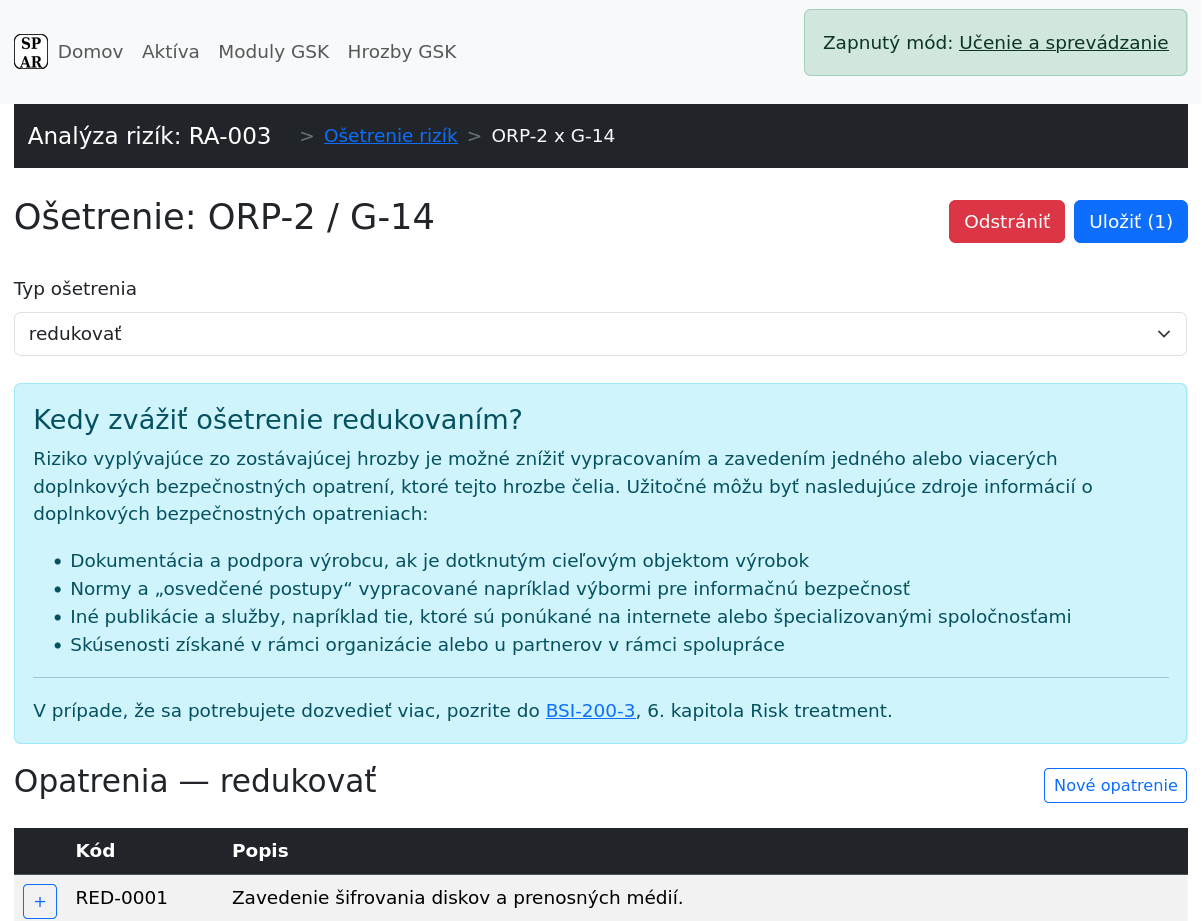
\includegraphics[width=0.6\textwidth]{images/learning-mode.png}
\caption{Ukážka používateľského rozhrania s inštruciami pri výbere ošetrenia redukovaním pre hrozbu a modul.}
\label{fig:learnmode}
\end{figure}

Vzhľadom na to, že ide o \emph{proof-of-concept}, nevideli sme pridanú hodnotu mať duplicitný text v používateľskom rozhraní a texte práce. Možno by bolo
užitočné investovať úsilie a zdroje do interaktívneho náučného rozhrania. Ešte spomenieme stránky modulov a hrozieb \cite{GSK}, ktoré by mohli poskytnúť
hlbšie informácie o moduloch a hrozbách, aby si užívateľ nemusel manuálne vyhľadávať potrebné informácie sám.


\section{Širší nadhľad na analýzu rizík}

Počas prieskumu a štúdia materiálov sme prečítali mnohé publikácie, ktoré sa venovali informačnej bezpečnosti alebo analýze/riadeniu rizík. Čitateľovi 
by sme niektoré z nich radi dali do pozornosti\footnote{Rozhodli sme sa sústrediť na štandardy BSI a \cite{GSK}, lebo nám narastal rozsah a došlo by ku
tzv. \emph{scope creep}.}, nakoľko súvisia s predmetom našej práce.

\cite{CyBOK} je príručka k súboru vedomostí o kybernetickej bezpečnosti, kde jednou z tzv. \enquote{knowledge area} (oblasť
vedomostí) tvorí \enquote{Risk Management \& Governance} (manažment a riadenie rizík). Napríklad, čitateľ získa náhľad do toho, ako vstupuje ľudský faktor
do riadenia rizík alebo to, ako navrhovať efektívne bezpečnostné opatrenia v súlade s ľudskou psychológiou; alebo do princípov riadenia rizika cez perspektívu
systému alebo komponentov (pozri \ref{fig:abstraction-hierarchy}). \cite{CyBOK} sme nakoniec do práce priamo nezakomponovali aj z dôvodu, že ide o
veľmi rozsiahly súbor teoretických poznatkov. 

\begin{figure}[ht]
    \centering
    \hspace*{-2.0cm}
    \begin{tikzpicture}[
        ahlevel/.style={
                rectangle,
                rounded corners=5pt,
                minimum width=8cm,
                minimum height=1.2cm,
                text width=7cm,
                align=center,
                font=\sffamily\bfseries,
                draw=#1!60!black,
                top color=#1!15,
                bottom color=#1!35,
                text=#1!15!black,
                line width=0.7pt,
            },
        linklabel/.style={
                font=\sffamily\footnotesize\itshape,
                text=gray!50!black,
                fill=white,
                inner sep=2pt,
                rounded corners=2pt,
            },
        sidelabel/.style={
                font=\sffamily\footnotesize,
                text=#1,
                rotate=90,
            },
        desc/.style={
                font=\sffamily\footnotesize,
                text=gray!50!black,
                anchor=west,
                text width=4.0cm,
            },
        desc2/.style={
                font=\sffamily\normalsize,
                text=#1,
                anchor=west,
                text width=4.5cm,
            },
        ]

        % Hierarchy levels (top to bottom)
        \node[ahlevel=Orange](L5) at (-1.0, 5.4) {Funkčný účel};
        \node[ahlevel=Orange](L4) at (-1.0, 3.6) {Abstraktná funkcia};
        \node[ahlevel=Orange](L3) at (-1.0, 1.8) {Zovšeobecnená funkcia};
        \node[ahlevel=Green] (L2) at (-1.0, 0.0) {Fyzická funkcia};
        \node[ahlevel=Green] (L1) at (-1.0,-1.8) {Fyzická forma};

        % Descriptions (right side)
        \node[desc] at (3.0, 5.4)
        {Účel alebo ciele systému};
        \node[desc] at (3.0, 3.6)
        {Princípy toku, rovnováhy a riadenia};
        \node[desc] at (3.0, 1.8)
        {Procesy, interakcia komponentov};
        \node[desc] at (3.0, 0.0)
        {Schopnosti, zaradenia a komponenty};
        \node[desc] at (3.0,-1.8)
        {Dimenzie a fyzikálne vlastnosti prostredia};

        \draw[loosely dotted, line width=2pt, color=black]
        (-6.0, 0.9) -- (11.6, 0.9);


        % left Side labels
        \node[sidelabel=Orange, anchor=south] at (-5.2, 3.6)  {koncepčná rovina};
        \node[sidelabel=Green, anchor=south] at (-5.2,-0.9)  {skutočná/reálna rovina};

        % left Side arrows (means-ends)
        \draw[{Stealth[length=2.5mm]}-{Stealth[length=2.5mm]}, line width=0.8pt, color=Orange!40]
        (-5.2, 6.3) -- (-5.2, 0.9);
        \draw[{Stealth[length=2.5mm]}-{Stealth[length=2.5mm]}, line width=0.8pt, color=Green!40]
        (-5.2, 0.9) -- (-5.2, -2.7);

        % right Side arrows (means-ends)
        \draw[{Stealth[length=2.5mm]}-{Stealth[length=2.5mm]}, line width=0.8pt, color=Orange!40]
        (7.5, 6.3) -- (7.5, 0.9);
        \draw[{Stealth[length=2.5mm]}-{Stealth[length=2.5mm]}, line width=0.8pt, color=Green!40]
        (7.5, 0.9) -- (7.5, -2.7);

        % left side labels
        \node[desc2=Orange] at (7.5, 3.6)
        {\textbf{systemovo-orientovaná analýza rizík}};
        \node[desc2=Green] at (7.5, -0.9)
        {\textbf{komponentovo-orientovaná analýza rizík}};

    \end{tikzpicture}
    \caption{Rasmussenova hierarchia abstrakcie}
    \label{fig:abstraction-hierarchy}
\end{figure}

Za zmienku stojí určite americký NIST a ich séria dokumentov \emph{special publications} (špeciálne publikácie), ktoré sú primárne zamerané na informačnú bezpečnosť
federálnych agentúr. \cite{NIST-800/39} sprevádza manažmentom rizík v tzv. enterprise (podnikovej) architektúre, ktorá je súčasťou \emph{enterprise risk management}.
\cite{NIST-800/53} je americkým ekvivalentom katalógu \cite{GSK}, v ktorom môžme nájsť zoznam 20 rodín a zoznamom navrhovaných bezpečnostných opatrení s diskusiou,
možnými rozšíreniami a vzťahmi s inými bezpečnostnými opatreniami. Okrajovo sme narazili ešte na \emph{Cybersecurity framework} \cite{CSF}, ktorý má údajne
zjednodušiť\footnote{V kontraste so zložitými špeciálnymi publikáciám, ako aj tie, ktoré sme my zmienili v tomto texte.} organizáciám pripraviť sa na kybernetické
hrozby v šiestich jadrových funkciách: riadiť, identifikovať, chrániť, zisťovať, reagovať a obnoviť. \cite{NIST-800/39} ani \cite{NIST-800/53} sme nakoniec do práce
nezahrnuli, nakoľko pokrývajú rovnakú problematiku ako Grundschutz a štandardy BSI, ale vychádzajú z (právnych, organizačných) podmienok v USA, ktoré sa líšia od tých
v Európskej únii\footnote{Spomínané publikácie obsahujú veľké množstvo manažérskych princípov, menej technických informácií, sú veľmi zdĺhavé a často idú do prílišných
podrobností, ktorým by čitateľ so základnými vedomosťami KIB aj tak neporozumel.}.

\section{Zakomponovanie bezpečnostných incidentov}

V kapitole \ref{chap:it-grundschutz} sme spomínali, že ISMS revidujeme v pravidelných intervaloch alebo vo výnimočných situáciach. Jednou z nich sú bezpečnostné
incidenty, ktoré môžu byť spúšťačom ďalšieho procesu analýzy rizík. Otázka znie, ako by sme mohli zakomponovať informáciu o bezpečnostných incidentoch, ktoré
sa v organizácii vyskytli? Budeme uvažovať hrozbu alebo zraniteľnosť, ktorá bola využitá? Upozorníme používateľa, aby v kroku, kedy ošetruje riziko, zaviedol
bezpečnostné opatrenia minimalizujúce pravdepodobnosť/dopad opakovaného incidentu? Prinútime dodatočne používateľa posúdiť ošetrenie bezpečnostného incidentu v
kroku \enquote{IT-Grundschutz check}?

\section{Vizualizácia získaných informácií}

Pri prezentovaní návrhu nášho systému v kapitole \ref{chap:application} čitateľ mohol vidieť rôzne maticové zobrazenia a tabuľkové sumarizácie dát. Sú to jednoduché
zobrazenia, ktorým sme určite nič nepokazili. Dovolíme si načrtnúť jeden z nápadov, ktorý sme mali na zjednodušenie vizualizácie pre používateľa môžeme vidieť na
obrázku \ref{fig:bread}. Preskúmať možné zobrazenia hrozieb, rizík a opatrení môže byť zaujímavým problémom v prípade vývoja komerčného produktu.

\begin{figure}[h!]
\centering
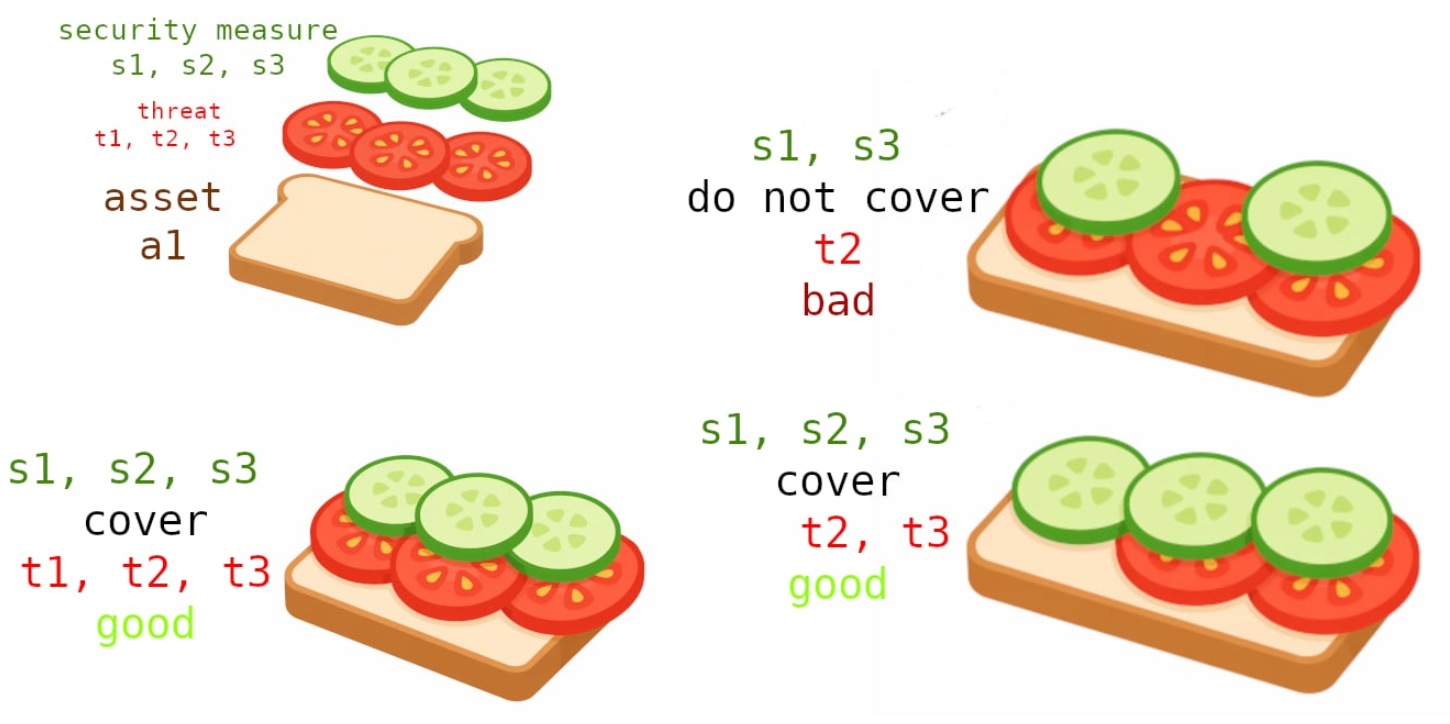
\includegraphics[width=0.6\textwidth]{images/bread.png}
\caption{Obložený chlebík, návrh zobrazenia pokrytia aktív (hnedá, chlieb), hrozieb (červená, paradajka) a opatrení (zelená, uhorka).
Vľavo hore vidíme jednotlivé úrovne prísad, vľavo dole vidíme kompletné pokrytie, vpravo hore nedostatočné pokrytie a vpravo dole nadbytočné pokrytie.}
\label{fig:bread}
\end{figure}

\section{Automatické upozornenie na aktívne hrozby}

Včasná reakcia na novo objavené hrozby je kľúčová pre minimalizáciu potenciálnych škôd v organizácií. Manažéri KIB môžu využiť stránku národného CSIRT
(\emph{Computer Security Incident Response Team}) \href{https://csirt.sk/index.html}{csirt.sk}, ktorý publikuje zoznam najnovších hrozieb s odporúčaniami,
ako ich ošetriť. V informačnom systéme môžeme tento proces zautomatizovať využitím jazyka a protokolu STIX/TAXII\footnote{
\emph{Structured Threat Information Expression}/\emph{Trusted Automated Exchange of Intelligence Information}}, ktoré sú určene na automatickú výmenu
informácií o kybernetických hrozbách. V našom systéme by sa klient pripojil na špecifikovaný server\footnote{K dispozícií sú verejné servery, ale aj platené,
ako to je v prípade \emph{ESET Threat Intelligence}.} a na relevantné hrozby by upozornil používateľa.

\section{Grundschutz++}

Snaha BSI a IT-Grundschutz zvýšiť bezpečnostnú úroveň organizácií a štátnych inštitúcií v Nemecku aj napriek dlhoročnej snahe nepriniesla očakávané výsledky.
V lete 2025 vrámci konferencie \emph{IT-Grundschutz-Tag} predstavitelia BSI priznali nedostatky \cite{GSK}, jedna z kritík sa týka orientácie \cite{GSK} na
komponenty. Iniciatívou a víziou \emph{Grundschutz++} má byť zmena orientácie na procesy, kedy si organizácia môže sledovať postup implementácie ISMS.
Prezentované boli aj mnohé ďalšie zmeny a zlepšenia (aj ako odpoveď na požiadvky \cite{NIS2}). To znamená, že môžeme očakávať výrazné zmeny súčasného
\cite{GSK} a jeho štandardov a časom možno aj novú metodológiu a nové štandardy.